\chapter{Completing Decode}


\begin{wrapfigure}{l}{1.5in}
\caption{iDecode}\label{fig:decode}
\begin{center}
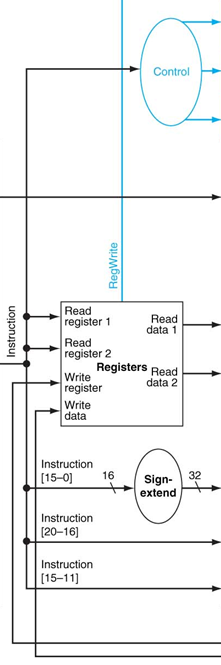
\includegraphics[width=1.5in]{../images/pipeline_decode.png}
\end{center}
\end{wrapfigure}

\WrapBarrier

\section{Buffer}

Buffers are a pretty simple concept, so I won't spend a lot of time on it.  I am giving you the entire buffer code from this stage (no delay included or needed).  Your key part will be in testing and incorporating it.

\section{Instruction Decode}


Probably the biggest job will thus be creating your instances of each element and hooking them up.  I have given you the basic code, but did not connect them.  All the wires needed are already made, so it should be straightforward to hook them up.  You will need to consult Figure~\ref{fig:decode}, to do the hooking up.  Note many signals come from the portions of the IR, based on the command type (R, I, J) and the corresponding bits of the field you want to access.  In some cases (particularly the outputs), you will need to refer to the fields by their names (RT, RD).  Don't forget that all outputs of the stage must be driven by the buffer, so they are timed correctly!  The line coming across between the control and register file is nPC - it just passes through, and will be used in execute to calculate the branch target.

\clearpage
\section{Your Assignment}

You are to:
\begin{enumerate}
\item Write a buffer for the outputs of the decode stage.
\item Write a testbench for the buffer, run a simulation and generate a timing diagram.
\item Integrate the control, sign extender, register file, and buffer into iDecode.
\item Write a testbench for the iDecode, run a simulation and generate a timing diagram.
\item  Write up a lab report in \LaTeX\ following the lab format in \verb1LabN.tex1 and generate a pdf file.
\item Upload the pdf and all the Verilog files to the course LMS.
\end{enumerate} 